\documentclass[11pt,a4paper]{article}
\usepackage[T1]{fontenc}
\usepackage[utf8]{inputenc}
\usepackage{lmodern}
\usepackage[margin=2.5cm]{geometry}
\usepackage{amsmath,amssymb}
\usepackage{booktabs}
\usepackage{multirow}
\usepackage{adjustbox}
\usepackage{graphicx}
\usepackage{xcolor}
\usepackage[font=small,labelfont=bf]{caption}
\usepackage[numbers,sort&compress]{natbib}
\usepackage{microtype}
\usepackage[colorlinks,linkcolor=blue!50!black,citecolor=blue!50!black,urlcolor=blue!50!black]{hyperref}
\newtheorem{proposition}{Proposition}

% Numbers that come from results/*.csv (benchmark, leakage audit) are written to generated/numbers.tex by build.py.
\newcommand{\LeakText}{A row-wise split lowers the error by a factor of 1.2--1.8, and copying the label of the nearest training cycle, without using any feature, gives 0.01--0.15 times the error of the model evaluated correctly, as the bound of Section~\ref{sec:data} predicts. Per-cell min--max normalisation over the whole life, as in the PINN4SOH code, lowers the error on XJTU (0.80) and HUST (0.46), where all cells end at almost the same SOH and the normalised cycle index, the fraction of life already elapsed, nearly determines SOH; it raises the error on TJU (1.51) and MIT (2.76), where end-of-life SOH varies and the normalisation erases the absolute level of the features. Either way the number does not describe deployment, where the life of a cell is unknown. A whole-life outlier filter and a normaliser fitted with test cells have smaller effects, but are leaks as well. All further results use the leakage-free protocol.}
\newcommand{\LeakRowAbstract}{1.2--1.8}
\newcommand{\LeakMinmaxAbstract}{0.46--2.76}
\newcommand{\LeakMaxFactor}{2.8}
\newcommand{\BenchText}{PINN4SOH~\citep{wang2024} is the reference result on these four datasets. We reconstructed its 39 evaluation groups (one model per batch for XJTU and TJU, one per dataset for MIT and HUST with 23 and 20 fixed test cells, and few-shot runs with $K = 1, \dots, 4$ labelled cells for XJTU and HUST) from the \texttt{data path} lines of the training logs released with the code, and evaluate everything as the paper does: MAE per test cell, averaged over cells, runs and groups.

\paragraph{The released configuration.} The training logs record, for every epoch, the mean ``physics loss'' of the monotonicity term. In the first released version of the model this term is \path{relu(y2-y1).sum()}, computed from the labels of consecutive cycles only. In all 39 groups the logged value is one constant across all epochs of all ten runs, and in all of them it equals this expression evaluated on the training rows that the original data loader builds from our copy of the data (e.g.\ 0.043214 for the XJTU 2C batch). The term therefore adds a constant and no gradient: the published numbers come from a model trained with the data and PDE terms only. The match also shows that our reconstructed splits and data reproduce the training rows of every published group. Two later revisions replaced the term, first by \path{relu(u2-u1).sum()} and then by \path{relu((u2-u1)*(y1-y2)).sum()}, and the latest commit notes that the loss weights $\alpha$ and $\beta$ changed after a bug fix; the default weights in the released scripts no longer match those in the logs.

\paragraph{Re-running the original code.} We ran the released model and data-loading classes unchanged on the reconstructed splits, with ten seeded runs per group as in the paper and two versions of the model: the version that produced the published numbers, with the logged hyperparameters, and the current version with its default weights (Table~\ref{tab:bench}, Figure~\ref{fig:bench}). The original code needs pandas~1.x semantics; we used pandas~2.3, PyTorch~2 and CPUs, whereas the original runs used GPUs and older libraries. The re-run of the published version gives 1.04--1.19 times the published error on the four full datasets and 0.97--1.20 times in the few-shot settings. Per test cell, the re-run is significantly worse on 2 of the 4 full datasets. The standard deviation over runs is 4--34\,\% of the mean, so single runs differ by as much as these gaps. Since the training rows are identical, the remaining differences are hardware, library versions and random seeds; we could not reproduce the original environment and do not know which of them causes the systematic part. We therefore report both the published numbers and the re-run, and use the re-run for paired tests because it gives per-cell predictions under known conditions. 

\paragraph{Same splits, same preprocessing.} With the original preprocessing (whole-life $3\sigma$ filter on all columns including capacity, per-cell min--max normalisation of features and cycle index), PINN-hybrid in its fixed configuration ($\omega = \tfrac12$, $w = 10$, three seeds, no tuning on these splits) has 0.78--0.92 times the error of the re-run original code on the full datasets (significantly lower in 2 and higher in 0 of 4) and 0.31--0.67 times in the few-shot settings (lower in 4, higher in 0 of 8). Against the published numbers the ratios are 0.85--1.10 and 0.37--0.73. In the few-shot settings the unlabelled training cells enter the physics losses of our model, which is where the semi-supervised design pays off. The strongest model under these conditions, however, is not a PINN: a GBDT with the same preprocessing has 0.77--0.84 times the re-run error on the full datasets and 0.21--0.58 times in the few-shot settings, and is significantly lower than PINN-hybrid in 3 of the 12 settings (higher in 0; ratio 0.69--0.98). With per-cell min--max normalisation, the normalised cycle index is the fraction of life already elapsed, a feature that a tree exploits directly.

\paragraph{Without the leaks.} With our leakage-free preprocessing the same model has 0.63 (TJU), 0.23 (MIT), 1.65 (HUST) times the published error on the full datasets (per test cell significantly lower on 2 and higher on 1 of 4). The direction follows the leakage audit (Section~\ref{sec:leak}): the original preprocessing helps on datasets where the elapsed fraction of life determines SOH (HUST) and hurts where the absolute feature level matters (TJU, MIT). A comparison that changes the preprocessing therefore cannot separate the model from the protocol, and the published numbers on the few-shot settings, where knowing the elapsed fraction of life is almost knowing SOH, mostly reflect the normalisation.}
\newcommand{\BenchAbstract}{has 0.78--0.92 times the error of the re-run original code on the full datasets and 0.31--0.67 times in its few-shot settings}
\newcommand{\BenchDiscussion}{Three practical points follow. Reported numbers should come with per-cell errors and the exact splits, which made the comparison possible here; the logs released with PINN4SOH allowed us to reconstruct both. Released code should be the code that produced the numbers, or the differences should be listed: a constant loss term and changed weights alter the method that is being compared. And preprocessing that uses the whole life of a cell should be avoided, because its effect on the error depends on the dataset and can be large in either direction.}


\newcommand{\E}{\mathbb{E}}
\newcommand{\Lc}{\mathcal{L}}

\title{Semi-supervised physics-informed learning for lithium-ion battery state-of-health estimation
  with scarce capacity measurements: a leakage-free benchmark}
% TODO (tác giả): thêm giảng viên hướng dẫn / đồng tác giả và email liên hệ trước khi nộp.
\author{Quoc Thang Huynh\\[2pt]
  \small Faculty of Computer Science and Engineering,\\
  \small Ho Chi Minh City University of Technology (HCMUT),\\
  \small Vietnam National University Ho Chi Minh City, Vietnam}
\date{Draft, \today}

\begin{document}
\maketitle

\begin{abstract}
Estimating the state of health (SOH) of lithium-ion cells from charging data is a regression problem whose labels are
expensive: each label is a full reference discharge. We study how far physics-informed neural networks (PINNs) can
reduce that cost, and we do so under an evaluation protocol that avoids the leakage common in this literature. The
model is a semi-supervised PINN whose solution network predicts SOH from 16 charge-curve features and is tied to a
grey-box degradation rate that is non-negative by construction; its three physics losses do not use labels, so they
also act on cells whose capacity was never measured. On four public datasets (387 cells, three chemistries), with
cell-wise stratified cross-validation, causal outlier filtering and training-only normalisation, the semi-supervised
PINN has 0.39--0.90 times the per-cell mean absolute error (MAE) of an identical network trained on labels alone when
10\,\% of the cells are labelled, but 0.85--1.09 times at 70\,\%, and a well-tuned gradient-boosted tree (GBDT)
remains the strongest single model. Averaging three PINNs with a GBDT and smoothing the
result with a causal trend filter gives an estimator that is better than GBDT in 10 of 16 dataset--label settings,
and better than CNN, LSTM and Transformer baselines in 47 of 48 comparisons. A leakage audit shows that row-wise
splits make the error of the same model look \LeakRowAbstract\ times smaller, and that per-cell min--max
normalisation over the whole life changes it by a factor of \LeakMinmaxAbstract, depending on the dataset. We re-run the original code of PINN4SOH, a published PINN
benchmark on the same datasets, on its own splits and find that its published runs used a monotonicity term computed
from labels only, which contributes no gradient; under identical splits and preprocessing our hybrid estimator \BenchAbstract. Finally, counting
labels as capacity measurements rather than cells, measuring every training cell at 1.2--6.0\,\% of its cycles gives
0.85--0.93 times the error of fully labelling 30\,\% of the cells, and a few measurements of the cell in service,
combined through a learned update model, lower the error further. Code, splits and run configurations are released.
\end{abstract}

\noindent\textbf{Keywords:} lithium-ion battery; state of health; physics-informed neural network; semi-supervised
learning; data leakage; cross-validation; benchmark reproducibility; measurement budget.

\section{Introduction}

The state of health of a lithium-ion cell, its present capacity relative to the nominal one, decides when a cell is
derated, repurposed or replaced. Capacity is not observed during normal use; it is measured by a full discharge under
reference conditions, which takes hours and interrupts operation. Battery management systems therefore estimate SOH
from signals that are always available, most often from the shape of the charging curve, and learn the mapping from
cells whose capacity was measured~\citep{roman2021,hu2020joule,sulzer2021}. The cost of such a model is set by how many
measured cells, and how many measurements per cell, it needs.

Physics-informed neural networks~\citep{raissi2019,karniadakis2021} offer one way to need fewer labels: a loss that
encodes known behaviour, such as capacity not recovering on its own, can be evaluated on data without labels. For
batteries, PINNs have been used with empirical degradation laws and with learned dynamics~\citep{wang2024,wen2023,navidi2024}.
Whether the physics actually saves labels, and against which baselines, is less clear. Two issues make published
numbers hard to compare. First, the evaluation protocol: consecutive cycles of a cell are almost identical, so a random
split by cycle turns the task into interpolation along a trajectory whose labels are known, and normalising each cell
by statistics of its whole life gives the model the fraction of life already elapsed, which is not known in
service~\citep{kapoor2023}. Second, baselines: gradient-boosted trees are strong on tabular features~\citep{grinsztajn2022},
yet comparisons often include only neural networks.

This paper reports a systematic study under a protocol designed to remove both problems. Our contributions are:
\begin{enumerate}
\item A leakage-free protocol for SOH estimation (cell-wise, stratified five-fold cross-validation repeated with
  different shuffles; causal outlier filtering; normalisation fitted on training cells only; paired per-cell
  statistics), and an audit that quantifies four common leaks on the same model.
\item A semi-supervised PINN with a grey-box, non-negative degradation rate whose physics losses are label-free, and a
  comparison with nine baselines at 10--70\,\% labelled cells on four datasets.
\item A hybrid estimator (three PINNs, a GBDT and a causal trend filter) chosen on validation data only.
\item A re-examination of the PINN4SOH benchmark~\citep{wang2024}: we re-run its released code on its own splits,
  identify that the published configuration's monotonicity term carried no gradient, and compare under identical
  splits and preprocessing.
\item An analysis of the measurement budget, in which labels are counted as capacity measurements: sparse measurements
  on all cells versus full labels on a subset, and updating the estimate of a cell in service from a few measurements.
\end{enumerate}

\section{Related work}

Data-driven SOH estimation maps features of charge or discharge curves, impedance or relaxation voltage to
capacity~\citep{severson2019,zhu2022,roman2021}. Gaussian processes~\citep{richardson2017} and tree ensembles are common
for engineered features; recurrent, convolutional and attention models~\citep{zhang2018lstm,hochreiter1997,bai2018tcn,vaswani2017}
operate on sequences of cycles. Physics enters either through the model structure, e.g.\ equivalent circuits and
electrochemical models~\citep{doyle1993,plett2015}, or through the loss. PINN4SOH~\citep{wang2024} couples a solution
network with a learned dynamical model $u_t = G(\mathbf{x}, t, u, u_\mathbf{x}, u_t)$ and reports results on the four
datasets used here. \citet{wen2023} build PINNs around empirical degradation models, and physics-informed approaches
to degradation diagnostics are compared by \citet{navidi2024} and discussed by \citet{aykol2021}.
Semi-supervised SOH estimation without additional degradation experiments has been studied by~\citet{lu2023}. Leakage
in machine-learning-based science is documented broadly~\citep{kapoor2023}; for batteries, \citet{roman2021} stress
cell-level splits and careful pipelines. Our work combines these threads in one controlled comparison and adds an
explicit re-run of a published benchmark.

\section{Data and evaluation protocol}\label{sec:data}

\subsection{Datasets and features}
We use four public cycling datasets, all as released with PINN4SOH~\citep{wang2024}, which share one feature
extraction (Table~\ref{tab:data}): XJTU (55 NCM cells, six protocols), TJU~\citep{zhu2022} (130 NCA, NCM and NCM+NCA
cells at 25, 35 and 45\,\textdegree C), MIT~\citep{severson2019} (125 LFP cells, fast-charging protocols) and
HUST~\citep{ma2022} (77 LFP cells, multi-step discharge). Each cycle is described by 16 statistics of the
constant-current voltage and constant-voltage current segments of the charge (mean, standard deviation, kurtosis,
skewness, slope, entropy, charge and duration). The label is $y_{c,n} = Q_{c,n}/Q_\text{nom}$. The cycle index enters as
$t_n = n/1000$ with one constant for all cells; scaling by the life of each cell would reveal the future.

\begin{table}[t]\centering\small
\caption{Datasets after preprocessing. Protocols: distinct test conditions used for stratification. Life: number of recorded cycles (min / median / max).}\label{tab:data}
\begin{adjustbox}{max width=\textwidth}\begin{tabular}{llrrrcccc}\toprule
Dataset & Chemistry & Cells & Cycles & Protocols & Life & Initial SOH & Final SOH & $Q_\text{nom}$ (Ah) \\\midrule
XJTU & NCM & 55 & 22,431 & 6 & 110 / 392 / 942 & 0.83--1.00 & 0.78--0.89 & 2.0 \\
TJU & NCA, NCM, NCM+NCA & 130 & 56,697 & 9 & 25 / 377 / 1,246 & 0.88--0.98 & 0.66--0.90 & 3.5/2.5 \\
MIT & LFP & 125 & 82,450 & 3 & 36 / 622 / 2,156 & 0.95--1.00 & 0.82--0.97 & 1.1 \\
HUST & LFP & 77 & 144,224 & 1 & 1,123 / 1,855 / 2,672 & 1.06--1.12 & 0.80--0.82 & 1.1 \\
\midrule Total & & 387 & 305,802 & & & & & \\
\bottomrule\end{tabular}\end{adjustbox}\end{table}


\subsection{Preprocessing without future information}
A cycle is discarded if any feature is not finite or deviates from the previous 50 cycles of the same cell by more
than five robust standard deviations (median and interquartile range of that window, at least ten cycles of history).
The threshold removes 1.6\,\% of cycles, comparable to the 2.2\,\% removed by a whole-life $3\sigma$ filter, but uses
only the past. Features are z-scored with means and standard deviations of the training cells, labelled and
unlabelled; validation and test cells never enter the normaliser.

\subsection{Cell-wise stratified cross-validation}
All cycles of a cell belong to the same part. With random row-wise splits, a test cycle is on average
$\E[d] = 1/(1 - (1-q)^2)$ cycles from the nearest training cycle when a fraction $q$ of rows is used for training
(1.10 cycles at $q = 0.7$), so copying the label of the nearest training cycle has an error of at most $\E[d]$ times
the mean absolute change between consecutive cycles. We use $K = 5$ folds stratified by test protocol: cells are shuffled within protocols and
assigned to folds by a counter that runs across protocols, so every fold contains every protocol, every cell is
tested exactly once per repetition, and fold sizes differ by at most one cell. Of the remaining cells,
$\operatorname{round}(0.1N)$ are used for validation (early stopping and all selection) and the rest, 70\,\% of the
cells, for training. A label fraction $f$ marks
$\operatorname{round}(fN)$ training cells as labelled, following a fixed order, so the labelled sets are nested in $f$;
$f = 0.7$ uses all training cells. The other training cells keep their features and serve as unlabelled data. The
shuffle is repeated five times (three for the later experiments), and in fold $k$ of repetition $r$ every model uses the
same seed $100r + k$, the same cells and the same normaliser, so comparisons are paired by cell.

\subsection{Metric and statistics}
The primary metric is the per-cell MAE, $\mathrm{MAE}_\text{cell} = |\mathcal{C}|^{-1}\sum_c n_c^{-1}\sum_n
|\hat y_{c,n} - y_{c,n}|$, which gives each cell one vote; we report it in units of $10^{-3}$ SOH. Each cell's error is
averaged over repetitions before testing. Differences are tested with the two-sided Wilcoxon signed-rank test on
per-cell differences~\citep{wilcoxon1945}, with Holm correction across the four datasets~\citep{holm1979}; ratios of
mean errors come with 95\,\% percentile bootstrap intervals resampling cells. Because training sets of folds overlap,
we also report where conclusions survive the corrected resampled $t$-test of~\citet{nadeau2003}.

\section{Methods}\label{sec:methods}

\subsection{Semi-supervised PINN with grey-box kinetics}
The solution network $F_\varphi:\mathbb{R}^{17}\to\mathbb{R}$ (SiLU, 17--128--128--64--1) maps standardised features
and time to SOH, $u = F_\varphi(\tilde{\mathbf{x}}, t)$. Degradation follows
\begin{equation}\label{eq:rate}
\frac{\partial u}{\partial t} = -\,r(\tilde{\mathbf{x}}, u, T), \qquad
r = \operatorname{softplus}\big(G_\theta(\tilde{\mathbf{x}})\big)\,
e^{\lambda\,\mathrm{clip}(1-u,\,-0.5,\,1)}\,
e^{-\frac{E_a}{R_g}\left(\frac{1}{T} - \frac{1}{T_\text{ref}}\right)},
\end{equation}
with a small rate network $G_\theta$ (16--32--32--1), a knee coefficient $\lambda = \operatorname{softplus}(\lambda_\text{raw})$
and an Arrhenius term with $E_a = 10^4\operatorname{softplus}(e_\text{raw})$\,J/mol. Every factor is positive, so
$r \ge 0$ for any parameters and every solution of \eqref{eq:rate} is non-increasing in $t$. For pairs of cycles
$(n_1, n_2)$ of one cell with $n_2 - n_1 \sim \mathcal{U}\{5,\dots,50\}$ and $u_i = F_\varphi(\tilde{\mathbf{x}}_{n_i}, t_{n_i})$,
\begin{align}
\Lc_\text{data} &= \overline{(u - y)^2}\quad\text{(labelled cycles only)}, &
\Lc_\text{ode} &= \overline{\big(\partial_t u_1 + r(\tilde{\mathbf{x}}_{n_1}, u_1, T)\big)^2}, \\
\Lc_\text{mono} &= \overline{\operatorname{ReLU}(u_2 - u_1 - \varepsilon)}, &
\Lc_\text{range} &= \overline{\operatorname{ReLU}(u_1 - 1.15) + \operatorname{ReLU}(0.4 - u_1)},
\end{align}
where the bar denotes the mean over a batch, $\varepsilon = 0.002$ and $\partial_t u$ comes from automatic
differentiation; at the first cycle of a cell,
$\Lc_\text{range}$ uses the tighter bounds $[0.85, 1.10]$. The loss is
$\Lc = \Lc_\text{data} + w(s)(\alpha\Lc_\text{ode} + \beta\Lc_\text{mono} + \gamma\Lc_\text{range})$ with
$\alpha = 0.02$, $\beta = 0.5$, $\gamma = 1$ and a linear warm-up $w(s) = \min(1, s/800)$. None of the three physics
losses contains $y$, so they are evaluated on pairs drawn half from labelled and half from unlabelled training cells
(PINN-semi). PINN-sup applies them to labelled cells only.

The physics here is phenomenological: capacity does not recover by itself, ageing accelerates as SOH falls, side
reactions follow Arrhenius kinetics, and SOH stays in a plausible range. It shapes the learned function; at inference
only $F_\varphi$ is evaluated (Figure~\ref{fig:arch}).

\begin{figure}[t]\centering
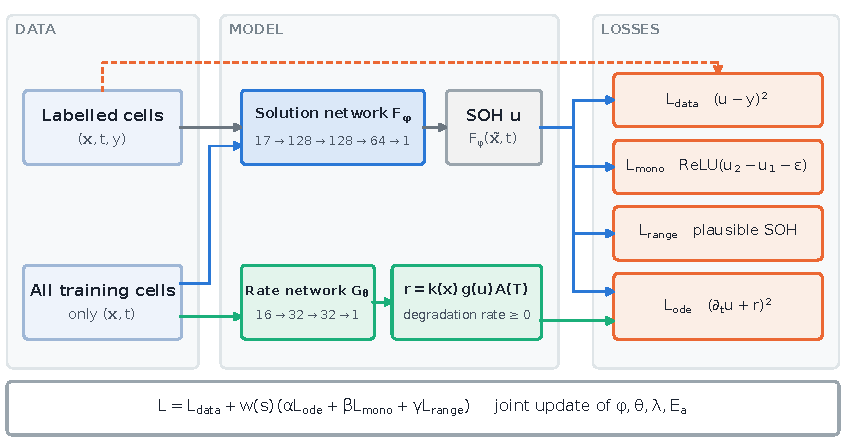
\includegraphics[width=\textwidth]{figures/fig_arch.pdf}
\caption{Semi-supervised PINN. The solution network predicts SOH from charge features and time; the rate network and
the knee and Arrhenius factors define a non-negative degradation rate. The data loss uses labelled cells only; the
monotonicity, range and kinetics losses use pairs of cycles from all training cells, labelled or not.}
\label{fig:arch}
\end{figure}

\subsection{Hybrid estimator}
The residual error of single models is dominated by a level offset per cell and slow drift
(Section~\ref{sec:hybrid}), which suggests averaging models whose per-cell offsets differ. The hybrid estimator, called
PINN-hybrid below, is
\begin{equation}\label{eq:hybrid}
\hat y_n = \omega\,\tfrac13\textstyle\sum_{m=1}^{3} F_{\varphi_m}(\tilde{\mathbf{x}}_n, t_n) + (1-\omega)\,g(\tilde{\mathbf{x}}_n, t_n),
\qquad
\tilde y_n = \bar y + \min(0, \hat\beta)(t_n - \bar t),
\end{equation}
where $F_{\varphi_m}$ are three PINN-semi networks that differ only in their seed, $g$ is the GBDT baseline trained on
the same labelled cells, and the second step fits a line with non-positive slope to the last $w$ predictions of the
cell and evaluates it at $t_n$ (a causal trend filter that does not use labels). The configuration
$\omega = \tfrac12$, $w = 10$ was fixed on validation data at repetition 0 with 10 and 50\,\% labels before any test
prediction was read; candidates that were rejected on validation include distillation from the GBDT, a stronger
monotonicity weight, an Euler residual along the trajectory and features relative to the first cycles. A tuned variant
selects $(\omega, w)$ from $\{0.3,\dots,0.7\}\times\{5, 10, 20, 40\}$ on the validation cells of each dataset and label
fraction.

\subsection{Baselines}
All models use the same inputs $[\tilde{\mathbf{x}}, t]$, splits, labelled cells and normaliser: ridge regression; a
Gaussian process with RBF and white-noise kernels on 1\,500 labelled points~\citep{rasmussen2006}; a histogram GBDT~\citep{friedman2001,ke2017}
with the number of trees chosen on validation; an MLP with the architecture of $F_\varphi$ trained on $\Lc_\text{data}$;
causal CNN, LSTM and Transformer models over the last $L$ cycles of the cell ($L = 16, 48, 16$, chosen on validation);
PINN-sup; and a black-box PINN with PINN4SOH-type dynamics $u_t = G(\mathbf{x}, t, u, u_\mathbf{x}, u_t)$ and the same
label-free losses. Networks are trained with AdamW~\citep{loshchilov2019} ($2\cdot10^{-3}$, cosine decay over 4\,000
steps), batches of 512 labelled points and 512 cycle pairs, and early stopping on validation MAE. Physics weights were
chosen once on validation in a preliminary experiment and kept fixed; no hyperparameter was chosen on test data.

\subsection{Measurement budget and updates in service}\label{sec:budgetmethods}
\emph{Sparse labels.} Instead of labelling every cycle of some cells, every training cell is measured at its first
cycle, every $qL$ cycles ($L$ is the median life of the training cells, $q \in \{0.5, 0.2, 0.1, 0.05\}$) and at its
last cycle. PINN-semi then uses $\Lc_\text{data}$ on measured cycles only while the physics losses still act on all
cycles; the GBDT learns linearly interpolated labels.

\emph{Kalman update.} When the cell in service is also measured occasionally, the error of the estimate $p_n$ is
modelled as $y_n - p_n = b_n + \varepsilon_n$: a cell-specific offset that drifts back to its mean as an
Ornstein--Uhlenbeck process, $b_{n'} - \mu_0 = e^{-(n'-n)/\ell}(b_n - \mu_0) + \eta$, plus fast noise with
$\operatorname{Var}\varepsilon = R$. A Kalman filter updates $b$ at each measurement and only uses measurements up to
the current cycle; $\mu_0$, $R$ and the stationary variance are estimated on the validation cells of the
fold and $\ell$ is chosen on a grid per measurement schedule.

\emph{Learned update.} The filter only corrects the offset of a model trained without measurements of the cell. The
learned update model instead predicts the change since the last measurement $m$, $\hat y_n = y_m + h(\mathbf{u}_n)$,
where $h$ is a GBDT on the current features, the change of features since $m$, $y_m$, the number of cycles since $m$
in units of $L$, and the slope between the last two measurements. It is trained on pairs drawn from the labelled
training cells under the test-time measurement schedules, with random phases.

\section{Results}\label{sec:results}

\subsection{Leakage audit}\label{sec:leak}
The same MLP at 70\,\% labels was trained under four protocols that each change one element of the leakage-free
protocol (Table~\ref{tab:leak}). \LeakText

\begin{table}[t]\centering\small
\caption{Leakage audit: ratio of the per-cell MAE of the same MLP (70\,\% labels) under each faulty protocol to its MAE under the leakage-free protocol (below 1: the error looks smaller than it is).}\label{tab:leak}
\begin{adjustbox}{max width=\textwidth}\begin{tabular}{lcccc}\toprule
Dataset & row-wise split & per-cell min--max & whole-life $3\sigma$ filter & normaliser incl.\ test \\\midrule
XJTU & \multirow{4}{*}{0.56--0.83} & 0.80 & \multirow{4}{*}{0.87--1.01} & \multirow{4}{*}{0.98--1.03} \\
TJU &  & 1.51 &  &  \\
MIT &  & 2.76 &  &  \\
HUST &  & 0.46 &  &  \\
\bottomrule\end{tabular}\end{adjustbox}\end{table}


\subsection{Label efficiency of the semi-supervised PINN}\label{sec:labels}
Table~\ref{tab:labels} gives the per-cell MAE of all single models at four label fractions. With 10\,\% labelled
cells (6--13 labelled cells per fold), PINN-semi has 0.60 (XJTU), 0.90 (TJU), 0.39 (MIT) and 0.61 (HUST) times the
error of the MLP, significantly lower on all datasets; at 30\,\% the ratio is 0.76--0.96, still significant on all four
but robust to the conservative fold-level test only on MIT. With 70\,\% labels, when no unlabelled cell is left and
PINN-semi equals PINN-sup, the ratio is 0.85--1.09; on TJU the MLP is significantly better. The geometric mean of the
ratio over datasets is 0.60, 0.86, 0.92 and 0.96 at 10, 30, 50 and 70\,\% labels (Figure~\ref{fig:labels}). Expressed
as labels saved, PINN-semi with 10\,\% labels matches an MLP trained on 17--45\,\% of the cells.

\begin{table}[t]\centering\small
\caption{Per-cell MAE ($\times10^{-3}$) on test cells at four fractions of labelled cells; five repetitions $\times$ five folds, every cell tested five times. Bold: lowest per dataset and column.}\label{tab:labels}
\begin{adjustbox}{max width=\textwidth}\begin{tabular}{llrrrr}\toprule
Dataset & Model & 10\,\% & 30\,\% & 50\,\% & 70\,\% \\\midrule
XJTU & Ridge & 18.22 & 15.54 & 14.81 & 14.09 \\
 & GPR & 14.85 & 12.11 & 14.86 & 19.18 \\
 & GBDT & \textbf{14.49} & \textbf{10.85} & \textbf{10.19} & \textbf{9.51} \\
 & MLP & 24.72 & 15.95 & 14.58 & 12.74 \\
 & PINN-sup & 20.25 & 14.54 & 13.21 & 12.19 \\
 & Black-box PINN & 15.68 & 14.15 & 12.82 & 12.34 \\
 & PINN-semi & 14.93 & 13.44 & 13.52 & 12.19 \\
\addlinespace
TJU & Ridge & 23.01 & 21.60 & 20.50 & 20.74 \\
 & GPR & 13.50 & 9.22 & 8.01 & 8.17 \\
 & GBDT & \textbf{12.68} & \textbf{8.14} & \textbf{7.21} & \textbf{6.77} \\
 & MLP & 15.50 & 11.33 & 9.99 & 9.64 \\
 & PINN-sup & 14.73 & 10.67 & 10.20 & 10.52 \\
 & Black-box PINN & 13.90 & 10.91 & 10.36 & 10.16 \\
 & PINN-semi & 13.91 & 10.85 & 10.46 & 10.52 \\
\addlinespace
MIT & Ridge & 3.53 & 3.24 & 3.17 & 3.13 \\
 & GPR & 3.21 & 2.14 & 1.84 & 1.79 \\
 & GBDT & \textbf{3.09} & \textbf{1.99} & \textbf{1.73} & \textbf{1.58} \\
 & MLP & 8.54 & 3.40 & 3.04 & 2.86 \\
 & PINN-sup & 5.34 & 2.69 & 2.54 & 2.44 \\
 & Black-box PINN & 4.19 & 2.80 & 2.61 & 2.54 \\
 & PINN-semi & 3.34 & 2.58 & 2.48 & 2.44 \\
\addlinespace
HUST & Ridge & \textbf{22.88} & 18.85 & 18.32 & 18.10 \\
 & GPR & 28.82 & 21.24 & 18.50 & 17.22 \\
 & GBDT & 24.13 & 18.63 & \textbf{15.65} & \textbf{14.45} \\
 & MLP & 37.95 & 19.80 & 17.73 & 16.94 \\
 & PINN-sup & 31.67 & 17.82 & 16.11 & 15.99 \\
 & Black-box PINN & 24.04 & 17.49 & 16.47 & 15.99 \\
 & PINN-semi & 22.98 & \textbf{17.30} & 16.11 & 15.99 \\
\bottomrule\end{tabular}\end{adjustbox}\end{table}


\begin{figure}[t]\centering
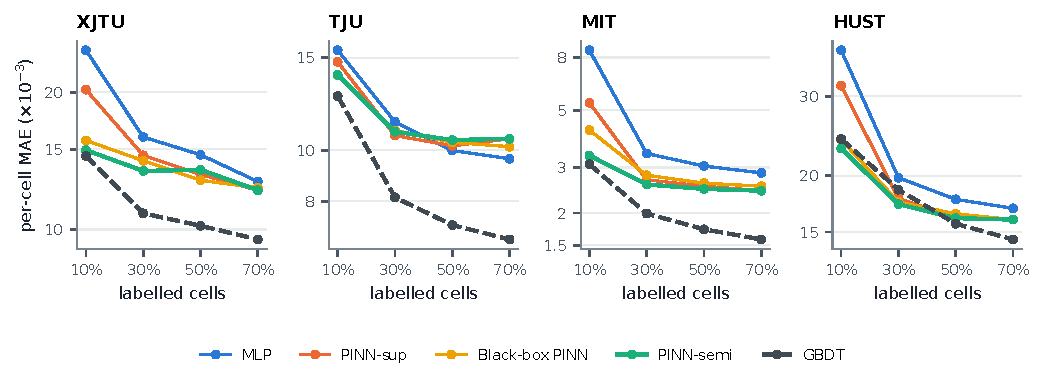
\includegraphics[width=\textwidth]{figures/fig_labels.pdf}
\caption{Per-cell MAE against the fraction of labelled cells (log scale). The semi-supervised PINN closes most of the
gap between the MLP and the GBDT at 10\,\% labels; with more labels, the GBDT stays lower on XJTU, TJU and MIT.}
\label{fig:labels}
\end{figure}

The GBDT is the strongest single model: it is better than PINN-semi in 14 of 16 settings, 10 of them significantly; the
reverse holds significantly only on HUST at 30\,\% labels. A Gaussian process is also lower than PINN-semi in 10 of 16
settings. The accurate statement is therefore that physics substantially improves the neural network when labels are
scarce, bringing it to within 0.95--1.10 times the GBDT at 10\,\% labels, but does not beat a well-tuned tree on most
datasets.

\paragraph{Where the gain comes from.} Table~\ref{tab:ablation} separates the components at 30\,\% labels. Applying the
physics losses to the unlabelled cells accounts for 50--64\,\% of the log-scale reduction relative to the MLP at
10\,\% labels; the rest comes from physics on labelled cells. At 30\,\% labels, the monotonicity loss alone provides
62--95\,\% of the reduction. The black-box dynamics of PINN4SOH perform almost exactly like monotonicity alone (within
2\,\%): when the dynamics network receives $u_t$ as input it can learn $G \approx u_t$ and satisfy the residual trivially,
an escape that the non-negative grey-box rate does not have. Measured on trained models at 30\,\% labels, MLP
predictions increase between cycles at least ten apart in 13.6--31.1\,\% of pairs and PINN-semi predictions in
3.0--12.0\,\%, close to the 0.1--7.7\,\% of the measured labels. Most of the predicted decline passes through the
charge features rather than through $t$. The learned $\lambda$ and $E_a$ stay at their initial values; on TJU, the only
dataset with several temperatures, raising the ODE weight fifty-fold or changing the initialisation moves them by
exactly the change of the initial value. With the rate written as $k(\mathbf{x})g(u)A(T)$, the feature-dependent factor
$k$ absorbs any change of $\lambda$ or $E_a$, so these parameters are structural, not identified.

\begin{table}[t]\centering\small
\caption{Source of the gain at 30\,\% labelled cells: per-cell MAE ($\times10^{-3}$) and, in parentheses, the ratio to the MLP.}\label{tab:ablation}
\begin{adjustbox}{max width=\textwidth}\begin{tabular}{lrrrr}\toprule
Model (30\,\% labels) & XJTU & TJU & MIT & HUST \\\midrule
MLP & 15.95 & 11.33 & 3.40 & 19.80 \\
PINN-sup (physics on labelled cells only) & 14.54 (0.91) & 10.67 (0.94) & 2.69 (0.79) & 17.82 (0.90) \\
PINN-semi, monotonicity only ($\alpha = \gamma = 0$) & 14.13 (0.89) & 11.00 (0.97) & 2.86 (0.84) & 17.41 (0.88) \\
PINN-semi, Euler residual along the trajectory & 13.37 (0.84) & 11.31 (1.00) & 3.01 (0.89) & 17.49 (0.88) \\
Black-box PINN (PINN4SOH-type dynamics) & 14.15 (0.89) & 10.91 (0.96) & 2.80 (0.83) & 17.49 (0.88) \\
PINN-semi & 13.44 (0.84) & 10.85 (0.96) & 2.58 (0.76) & 17.30 (0.87) \\
\bottomrule\end{tabular}\end{adjustbox}\end{table}


\subsection{Hybrid estimator and sequence models}\label{sec:hybrid}
At 30\,\% labels, the errors of the MLP, PINN-semi and GBDT are dominated by per-cell level offsets (14--58\,\% of
the MSE) and slow drift (32--57\,\%); fast cycle-to-cycle noise accounts for 1--17\,\% outside MIT. The per-cell offsets of the PINN ensemble and the GBDT are
only moderately correlated (Pearson 0.50--0.80) and have opposite signs for 16--31\,\% of the cells, which is why
averaging them helps. With the fixed configuration, PINN-hybrid has a lower MAE than PINN-semi in 16 of 16 settings (all
significant; ratio 0.67--0.95) and than the GBDT in 10 of 16 (8 significant), including all four datasets at 10\,\%
labels; the GBDT remains significantly better only on TJU at 70\,\%. On the two label fractions used during
development, the test ratio to PINN-semi (0.805) is close to the validation ratio (0.823), so selection on validation
did not make the test result optimistic. The geometric-mean ratio to PINN-semi falls to 0.961 with the ensemble, 0.798
with the GBDT and 0.793 with the filter; most of the gain comes from combining the two model families. With MLPs in
place of the PINNs (same GBDT and filter), the physics still helps at low label fractions (geometric-mean ratio 0.716
at 10\,\%) but not at 70\,\% (1.002).

Table~\ref{tab:main} adds the sequence models and the tuned hybrid on the same folds. Looking at several cycles helps
the neural networks: CNN, LSTM and Transformer reach 0.36--0.93 times the MLP error (significant in 42 of 48
comparisons) and beat PINN-semi in 14 of 16 settings, but they are worse than the GBDT in 40 of 48 and worse than
PINN-hybrid in 47 of 48 comparisons. The tuned hybrid is lower than the GBDT significantly in 11 of 16 settings and
never significantly higher. Adding causal feature history (exponential moving averages and recent slopes) helps on TJU
and HUST from 30\,\% labels but hurts on XJTU; selecting history per dataset and label fraction on validation (a post
hoc analysis, last column) gives a lower MAE than the GBDT in all 16 settings, 13 significantly.

\begin{table}[t]\centering\small\setlength{\tabcolsep}{4.5pt}
\caption{Per-cell MAE ($\times10^{-3}$) of the main models on the same folds and labelled cells (three repetitions $\times$ five folds). PINN-hybrid: weights and filter window tuned on validation. $^\dagger$Hybrid with or without causal feature history, selected on validation per dataset and label fraction (post hoc). Bold: lowest per row.}\label{tab:main}
\begin{adjustbox}{max width=\textwidth}\begin{tabular}{llrrrrrrrr}\toprule
Dataset & Labels & MLP & CNN & LSTM & Transformer & GBDT & PINN-semi & PINN-hybrid & + history$^\dagger$ \\\midrule
XJTU & 10\,\% & 23.27 & 16.01 & 16.62 & 17.63 & 14.01 & 14.65 & \textbf{12.71} & \textbf{12.71} \\
 & 30\,\% & 15.61 & 12.68 & 13.98 & 13.71 & 10.87 & 13.35 & \textbf{10.78} & \textbf{10.78} \\
 & 50\,\% & 14.10 & 11.69 & 11.98 & 12.05 & 10.18 & 13.20 & \textbf{10.02} & \textbf{10.02} \\
 & 70\,\% & 12.48 & 10.98 & 10.50 & 10.99 & 9.64 & 12.53 & \textbf{9.50} & \textbf{9.50} \\
\addlinespace
TJU & 10\,\% & 15.81 & 14.22 & 13.08 & 14.14 & 12.60 & 14.01 & \textbf{11.70} & \textbf{11.70} \\
 & 30\,\% & 11.71 & 8.89 & 8.69 & 9.89 & 8.06 & 11.39 & 8.00 & \textbf{7.78} \\
 & 50\,\% & 9.96 & 7.31 & 7.24 & 9.31 & 7.17 & 10.74 & 7.23 & \textbf{6.92} \\
 & 70\,\% & 9.71 & 7.36 & 7.09 & 8.96 & 6.96 & 10.80 & 7.11 & \textbf{6.82} \\
\addlinespace
MIT & 10\,\% & 9.02 & 3.30 & 3.26 & 3.87 & 3.15 & 3.29 & \textbf{2.52} & \textbf{2.52} \\
 & 30\,\% & 3.39 & 2.18 & 2.18 & 2.77 & 1.97 & 2.50 & \textbf{1.75} & \textbf{1.75} \\
 & 50\,\% & 3.06 & 1.99 & 2.04 & 2.71 & 1.74 & 2.45 & \textbf{1.59} & \textbf{1.59} \\
 & 70\,\% & 2.85 & 1.93 & 1.99 & 2.59 & 1.59 & 2.38 & \textbf{1.48} & \textbf{1.48} \\
\addlinespace
HUST & 10\,\% & 41.62 & 22.77 & 24.51 & 21.95 & 23.84 & 22.76 & \textbf{20.36} & \textbf{20.36} \\
 & 30\,\% & 20.00 & 17.42 & 17.14 & 17.45 & 18.73 & 17.10 & 15.99 & \textbf{15.34} \\
 & 50\,\% & 18.13 & 15.04 & 15.52 & 16.00 & 15.82 & 16.42 & 14.26 & \textbf{13.17} \\
 & 70\,\% & 17.19 & 14.19 & 14.76 & 14.93 & 14.60 & 16.38 & 13.76 & \textbf{12.24} \\
\bottomrule\end{tabular}\end{adjustbox}\end{table}


\subsection{Revisiting the PINN4SOH benchmark}\label{sec:bench}
\BenchText

\begin{table}[t]\centering\small\setlength{\tabcolsep}{4pt}
\caption{Per-cell MAE ($\times10^{-3}$) on the PINN4SOH splits, averaged over test cells, runs and groups as in the original paper. Re-runs: the released code, ten runs per group (seeds 0--9), as published (label-only monotonicity term, logged hyperparameters) and as currently released (corrected term, new defaults); $\pm$: standard deviation over runs. Ours: three seeds. $K$: labelled training cells in the few-shot experiments. $^{*}$/$^{\dagger}$: hybrid with the original preprocessing significantly lower/higher than the re-run as published (Wilcoxon over test cells, Holm across the 12 rows).}\label{tab:bench}
\begin{adjustbox}{max width=\textwidth}\begin{tabular}{llrrrrrr}\toprule
 & & \multicolumn{3}{c}{PINN4SOH} & \multicolumn{3}{c}{ours} \\\cmidrule(lr){3-5}\cmidrule(lr){6-8}
Dataset & Setting & published & re-run, as published & re-run, current & hybrid, orig.\ prep. & GBDT, orig.\ prep. & hybrid, leakage-free \\\midrule
XJTU & all cells & 7.85 & 8.77 $\pm$ 0.76 & -- & -- & -- & -- \\
TJU & all cells & 9.79 & 11.37 $\pm$ 2.14 & -- & -- & -- & -- \\
MIT & all cells & 6.18 & 7.50 $\pm$ 0.73 & -- & -- & -- & -- \\
HUST & all cells & 7.57 & 8.03 $\pm$ 0.95 & -- & -- & -- & -- \\
\addlinespace
XJTU & $K = 1$ & 31.54 & 35.15 $\pm$ 10.89 & -- & -- & -- & -- \\
 & $K = 2$ & 10.06 & 11.01 $\pm$ 1.54 & -- & -- & -- & -- \\
 & $K = 3$ & 7.98 & 8.97 $\pm$ 1.41 & -- & -- & -- & -- \\
 & $K = 4$ & 7.62 & 8.77 $\pm$ 0.41 & -- & -- & -- & -- \\
\addlinespace
HUST & $K = 1$ & 39.42 & 47.13 $\pm$ 15.83 & -- & -- & -- & -- \\
 & $K = 2$ & 16.94 & 18.07 $\pm$ 3.15 & -- & -- & -- & -- \\
 & $K = 3$ & 14.59 & 15.10 $\pm$ 1.41 & -- & -- & -- & -- \\
 & $K = 4$ & 13.62 & 14.62 $\pm$ 0.60 & -- & -- & -- & -- \\
\bottomrule\end{tabular}\end{adjustbox}\end{table}


\begin{figure}[t]\centering
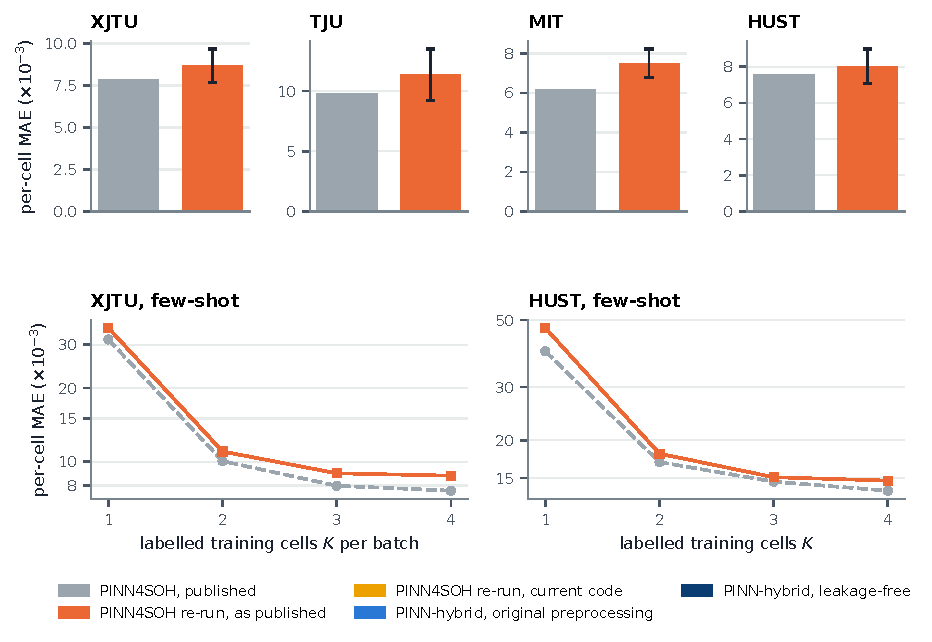
\includegraphics[width=\textwidth]{figures/fig_benchmark.pdf}
\caption{PINN4SOH splits. Top: full training sets, per dataset. Bottom: few-shot experiments with $K$ labelled cells
(XJTU per batch, HUST overall). Published: numbers released with PINN4SOH. Re-run: the released code, ten runs per
group, as published (label-only monotonicity term) and as currently released (corrected term). Ours: PINN-hybrid with
the original preprocessing and with the leakage-free preprocessing.}
\label{fig:bench}
\end{figure}

\subsection{Where to spend capacity measurements}\label{sec:budget}
Labelling every cycle of 30\,\% of the cells uses 43--44\,\% of the training cycles. Measuring all training cells every
$0.05L$ cycles uses 1.2--6.0\,\%, 7--37 times fewer, yet PINN-hybrid trained this way has a lower MAE than with 30\,\%
of the cells fully labelled on all four datasets (ratio 0.85--0.93, all significant) and 0.97--1.05 times the error with
70\,\% labelled (Table~\ref{tab:budget}). Consecutive cycles of a cell repeat each other's information, whereas the
dominant error, the level offset of each cell, can only be learned from labels of that cell; spreading measurements over
cells pays for that. The same holds for every model: a GBDT on interpolated labels at $0.05L$ is within 1.00--1.04 times
the GBDT with 70\,\% of the cells labelled. At the sparsest schedule ($0.5L$, about three measurements per cell), linear
interpolation misses the late acceleration, and on XJTU and MIT the GBDT on interpolated labels is up to three times
worse than the PINNs, whose monotonicity and kinetics losses connect the measurements.

\begin{table}[t]\centering\small\setlength{\tabcolsep}{4pt}
\caption{Measurement budget: per-cell MAE ($\times10^{-3}$) on test cells, three repetitions; in parentheses, the percentage of training cycles with a capacity measurement (70\,\% of the cells labelled is all of them). Sparse: every training cell measured at its first cycle, every $qL$ cycles and its last cycle. Last column: the cell in service is also measured every $0.1L$ cycles and the estimate is updated with the Kalman filter; error on unmeasured cycles.}\label{tab:budget}
\begin{adjustbox}{max width=\textwidth}\begin{tabular}{lrrrrrr}\toprule
 & \multicolumn{3}{c}{labels per cell} & \multicolumn{2}{c}{sparse, all cells} & sparse + in service \\\cmidrule(lr){2-4}\cmidrule(lr){5-6}\cmidrule(lr){7-7}
Dataset & Hybrid, 30\,\% & Hybrid, 70\,\% & GBDT, 70\,\% & Hybrid, $0.1L$ & Hybrid, $0.05L$ & Hybrid, $0.1L$ \\\midrule
XJTU & 11.43 (44.1) & 10.00 & 9.64 & 10.51 (3.2) & 10.28 (6.0) & 7.46 \\
TJU & 8.52 (42.6) & 7.76 & 6.96 & 8.28 (3.1) & 7.54 (5.9) & 4.13 \\
MIT & 1.79 (42.7) & 1.59 & 1.59 & 1.91 (1.9) & 1.67 (3.6) & 1.18 \\
HUST & 16.19 (43.1) & 13.78 & 14.60 & 13.87 (0.6) & 13.78 (1.2) & 5.00 \\
\bottomrule\end{tabular}\end{adjustbox}\end{table}


\paragraph{Updating a cell in service.} If the cell in service is also measured every $0.1L$ cycles (1--3\,\% of its
cycles) and the estimate is updated with the Kalman filter, the error on unmeasured cycles falls to 1.2--7.5 ($10^{-3}$),
0.34--0.77 times the GBDT trained with 70\,\% of the cells labelled and not updated; with the same schedule in
service, the hybrid trained with 70\,\% of the cells labelled gives 1.0--7.4, so once the cell is measured the training
labels matter little. A single measurement at commissioning helps little, because the capacity of many cells still rises
during the first tens of cycles. Across the four datasets, four label fractions and three sparse schedules,
the filter beats the uncorrected estimate in 46 of 48 cases and beats simply holding the last measured value in 48 of
48. When every previous cycle is measured, however, holding the last value is better than the filter (ratio of the
filter to holding 1.17--1.52): the cycle-to-cycle change predicted by the model is noisier than the true change. The
learned update model addresses exactly this: it is lower than the Kalman filter in 47 of 48 sparse settings (ratio
0.15--1.06) and lower than holding the last value in 48 of 48 (0.07--0.53); with every previous cycle measured it beats
the filter in 16 of 16 settings and is significantly lower than holding in 12 of 16 (significantly higher in one,
XJTU at 10\,\% labels).

\section{Discussion}\label{sec:discussion}

\paragraph{When does the physics help?} Among networks that see one cycle, the semi-supervised PINN should be preferred
when labelled cells are few (10--30\,\%) and many unlabelled cells exist; the gain comes from the label-free losses on
those cells, and most of it from the monotonicity constraint along real trajectories. When labels are plentiful, the
physics adds little. Trees remain strong on these engineered features, and the most useful role for the PINNs is as a
component that disagrees with the tree in a different way. Sequence models reach a similar improvement over the MLP by
another route, looking at the recent cycles of the cell, which suggests using a sequence model as the solution network
of a PINN.

\paragraph{Leakage changes conclusions, in both directions.} Row-wise splits always flatter the model. Per-cell
normalisation over the whole life is subtler: it reveals the elapsed fraction of life, which nearly determines SOH when
all cells end at similar SOH (XJTU, HUST), but erases the absolute level of the features, which carries information when
end-of-life SOH varies (TJU, MIT). Its effect on a reported number can therefore be an improvement or a degradation, and
neither reflects deployment, where the life of the cell is unknown.

\paragraph{Lessons from the benchmark re-run.} \BenchDiscussion

\paragraph{Limitations.} (i) Validation cells are fully labelled and lie outside the label budget in all experiments,
including the sparse-measurement ones. (ii) Physics weights were set once and not tuned per dataset. (iii) The physical
parameters $\lambda$ and $E_a$ are not identified by these data. (iv) The hybrid combines the models at the prediction
level; physics is not part of the tree. (v) Later experiments use three of the five repetitions. (vi) Variants marked
as tuned or post hoc were selected on validation data but defined after test results of the fixed versions were known.
(vii) Our re-run of PINN4SOH uses CPUs and recent library versions; run-to-run variation is reported, but the original
hardware and software could not be reproduced exactly. (viii) All data are laboratory cycling at controlled
temperature; field data with irregular measurements remain to be tested.

\section{Conclusion}
Under a leakage-free protocol on 387 cells, a semi-supervised PINN with label-free physics losses substantially improves
a neural network when few cells are labelled, but a tuned GBDT remains the strongest single model; averaging PINNs with
the tree and filtering the result causally gives the best estimator in most settings. Common preprocessing choices
change reported errors by factors of up to \LeakMaxFactor, in either direction, and a re-run of a published benchmark shows how
much released code, logged configurations and evaluation details matter. For deployment, the useful question is not how
many cells to label but where to place capacity measurements: sparse measurements on every cell, and a few
measurements of the cell in service, are worth more than full labels on a subset.

\section*{Data and code availability}
The datasets are public and were obtained from the PINN4SOH repository (commit \texttt{cc3cc50}). All code, the
reconstructed PINN4SOH splits, the run configurations and the scripts that produce every table and figure of this paper
are available in the accompanying repository; \texttt{python run.py all} reproduces the experiments, the benchmark
re-run and this manuscript.

\bibliographystyle{unsrtnat}
\bibliography{refs}
\end{document}
